\documentclass[12pt]{article}
\usepackage{graphicx}
\usepackage {color}
\usepackage{pdfpages}
\usepackage{float}
\usepackage{changebar}
\usepackage{enumitem,amssymb}
\renewcommand{\familydefault}{\sfdefault}
\usepackage[margin=1.2in]{geometry}
\usepackage{graphicx}
\usepackage{wrapfig}
\usepackage[super]{cite}
\usepackage{subcaption}
\usepackage[table]{xcolor}
\usepackage{amsmath}
\usepackage[sort, numbers]{natbib}
\usepackage{matlab-prettifier}
\usepackage{wrapfig,lipsum,booktabs}
%%%%%%%%%%%%Defining the margins %%%%%%%%%%%%%%%%%%%%%
\textheight 9.in
\textwidth 6.5in
\topmargin -.5in
\oddsidemargin 0in
\setlength{\parskip}{\smallskipamount}

%%%%%%%%%%%%%%Specific Commands %%%%%%%%%%%%%%%%%%
\newcommand{\eg}{{\em e.g.,}}
\newcommand{\ie}{{\em i.e.,}}
\newcommand{\etc}{{\em etc.,}}
\newcommand{\etal}{{\em et al.}}
\newcommand{\degrees}{{$^{\circ}$}}
\newcommand{\micro}{{$\mu$}}


%%%%%%%%%%%%%%%%%%%%%%%%%%%% Setting to control figure placement
% These determine the rules used to place floating objects like figures 
% They are only guides, but read the manual to see the effect of each.
\renewcommand{\topfraction}{.9}
\renewcommand{\bottomfraction}{.9}
\renewcommand{\textfraction}{.1}
\renewcommand{\familydefault}{\sfdefault} %setting the san serif font

%%%%%%%%%%%%%%%%%%%%%%%% Line spacing
% Use the following command for ``double'' spacing
%\setlength{\baselineskip}{1.2\baselineskip}
% and this one for an acceptable NIH spacing of 6lpi based on 11pt
%\setlength{\baselineskip}{.9\baselineskip}
% The baselineskip does not appear to work when we include a maketitle
% command in the main file.  Something there must set the line spacing
% If we use this next command, then things seem to work.
\renewcommand{\baselinestretch}{.9}

\setcounter{secnumdepth}{0} %make no numbers but have a table of contents


\begin{document}

\title{Lab 2, Propagation}
\author{Jake Bergquist, u6010393}
\maketitle
\tableofcontents
\newpage

\section{Introduction}
The body surface electrocardiogram (ECG) has been the most commonly used noninvasive technique for assessing the activity of the heart since it was made practical by Willem Einthoven in |?. The ECG leverages the fact that the heart is a bioelectriaclly active tissue whose electrical activity is directly tied to its function. When combined with the propagation of these electrical signals through an electrically passive conductive torso this electrical activity of the heart can be recorded remotely at the torso surface. Because of the direct relationship between cardiac electrical activity and its physiologic function, the ability to measure this activity in real time and noninvasively makes it a powerful clinical tool for assessing and diagnosing cardiac health. The particaly locations that are used to record from the torso surface play a key role in interpreting the signals derived from them. Originally willem Einthoven devised three major leads to record from using electrodes attached to the arms and one to the left leg. By making bipolar recording across these leads to form the Einthoven triangle consisting of leads I (-right arm +left arm), II (-right arm +left leg), and III (-left arm + left leg) researchers and clinicians can assess the major activity of the heart as electrical propagation projects onto these different recording leads. These leads however only provide general recordings of the heart activity, which is why several other lead sets exist. The most common of these is the 12 lead ECG, consisting of the 3 Einthoven leads (usually placed on shoulders and lower torso rather than on the limbs directly), 6 precordial leads arrange from just to the right of the sternum and stretching across toward the left maxillary line, as well as 3 ``computed'' leads that are mathematically derived from some combination of the other 9. The precordial leads are unipolar recordings with reference to Wilson's central terminal, which is constructed by averaging the three Einthoven leads. These unipolar leads are placed close to different regions of the heart as viewed from the torso surface and attempt to assess more local phenomena of the heart. For example, the usual placement of V1 (the first percordial lead) is closest to the right ventricle fo most hearts (assuming typical anatomy), thus alterations to the waveform seen on V1 can indicate changes in the electrical activity specifically of the right ventricle. One example would be during right bundle branch block, in which conduction is slowed in the right ventricle due to lack of right bundle and purkinje involement. Under these conditions V1 would see an aytypical all positive QRS deflection which V6 would see an atypical all negative QRS deflection. These changes indicate that propagation primarily moves towards the right ventricle, as is expected when conduction is slowed in that region. The Left ventricle activates quickly by comparison and thus the majority of the now extended activation sequence occurs as the right ventricle slowly activates. In this case the wavefront of activation moves up the right ventricle towards V1 (leading to a positive deflection) and away fro V6 (leading to a negative deflection). this is just one of many examples where changes in the signals seen on a body surface ECG can be used for cardiac diagnosis. 

As is the case with many biomedical domains, a powerful tool for investigation of different parameters in a disease state is simulation. Simulation environments allow for the manipulation of parameters in a biological system that are either impractical, impossible, or unethical to perform in eithe rhuman or animal experiments. Additionally simulation studys benefit from a lower cost than a typical experimental preparation as they require only a computer with sufficient resources to run the simulation of interest (although this can be a challenge of its own depending on model complexity). Int he case of ECG simulation these benefits also apply. A researcher can, for example, alter conduction patterns on the heart to match some disease state they wish to study, and simulate the resulting body surface potentials in order to assess how this disease state would change the clinical or full body surface ECG. The method by which this is done is called the cardiac forward problem, the projection of cardiac source signals onto the body surface. There are several approaches and formulations to addressing this problem but generally it is considered to be a well behaved system of equations, although this is still an area of active research. OVerall these solution methods seek to solve for the body surface signals resulting from some cardiac source by means of a transfer function. This transfer functiont akes into account the conductivity of the passive volume conductor of the torso and can also include conductivity inhomogeneities such as those introduced by bones or lungs. In order to construct such a transfer function the researcher must first identify the nature of the cardiac source. This cna come in the form of simulated transmembrane voltages of action potentials throughout the heart, such as those that could be obtained from a monodomain or bidomain formulation. Another bioelectric source formulation would be epicardial surface potnetials, as is the case in the boundary element potential forward problem. In this case a simple transfer matrix can be used to project cardiac source potentials to body surface potnetials by accounting for the solid angle contribution from primary (cardiac) and secondary (``reflected'' or torso) sources. Different source formulations result in differeng complexity for forward computation, and differing levels of control for manipulation of parameters.

ECGSim is a powerful research and educaton tool that leavarges the forward relationship of cardiacl electrophysiology in order to provide a robust platform for realtime analysis and investigation of the consequences of changes to underlying cardiac source behavior and the resultant body surface ECG. The core of ECGSim is built on the source model of transmembrane voltage efined on the endo and epicardial surfaces, and a boundary element formulation top calculate a forward transfer matrix. Because the transfer matrix can be calculated independently of the cardiac source signals and only depends on the description of the volume conductor (geometry and conductances) it can be precomputed. This allows changes in the cardiac source to be propagated to the body surface ECG in near real time. The key feature of ECGSim allows for dynamic and interactive exploration of how changes to the cardiac source result in changes in the measured ECG. ECGSim allows for changes to action potnetial morphology including changes of resting membrane potnetial, plateau potential, activation time, and recovery time. These changes can be made across the heart gewometry and can be varied heterogeneously. ECGSim comes with several prepared datasets and is available for the integration of novel datasets. The simulated signals can be visualized and interrogated in real time according to activation time, extracellular potential, transmembrane potnetial, recovery time, and activation recovery interval on the heart surface. On the body surface the body surface potential, activation map, and recovery map as well as a few other visualizations can be explored in rela time, in addition to the full simulated ECG signals from the 12 lead (and other) lead sets.

\section{Methods}
For all sections of this lab the default normal male case file was used. In between each lab section the default file was reloaded to prevent perturbations from previous sections from affecting subsequent ones.

\subsection{1.1: }
Using the default case I investigated the temporal sequence of activation. I visualized the activation times, as well as the transmembrane potentials and scrolled through time in order to watch the activation propagation. I noted what areas of the endo and epicardium activated first and last, and in what direction the propagation spread.
\subsection{1.2: }
Using the default case I investigated the temporal sequence of deactivation or repolarization. I visualized the recovery times, as well as the transmembrane potentials and scrolled through time in order to watch the recovery sequence. I noted what areas of the endo and epicardium recovered first and last and made comparisons to the observations of activation from section 1.1.
\subsection{1.3: }
Using the default case I investigated the arrangement and patterns of the extracellular cardiac potentials during the cardiac cycle. I visually assessed timepoints and locations of high potential gradient and observed the range and distributions of potentials during the cycle.

\subsection{2.1: }
I investigated the reconstruction of the 12 lead ECG in the ECG sim environment by examining the body surface potnetials through the heart beat. By using the vECGSim settings that visualize the lead placement for the simulated 12 lead electrode set I was able to interrogate how the body surface potential map translated tot he 12 lead ECG signals displayed.

\subsection{2.2: }
 In order to investigate changes to the action potential duration and how they would effect the resultant ECG I modified the action potential duration of the left ventricular free wall by $\pm$25\% and $\pm$50\% . I used the single node selection tool and set the changes to be transmural. I then set the area of effect to cover most of the left ventricular free wall. I oberved and documented hte resulting changes to the ECG signals at each of these perturbations. In particular I assessed changes to the waveform measured by Einthoven lead I. 
 
 \subsection{2.3: }
 In order to simulate left bundle branch block I altered the activation times of the tissue transmurally int he left ventricle starting at the basal free wall. This region should have the latest activation in the case of left bundle branch block, and thus I delayed activation here by roungly 100 ms. Using the multi-node select tool and a small area of effect I incrementally adjusted actvation times down the left ventricular free wall towards the septum to create a gradient of activation starting at the septum and ending at the basal left ventricular free wall. I then assessed the resulting changes to the ECG under these conditions.
 
 
\section{Results}
\subsection{1.1: }
The activation times mapped onto the endocardium and epicardium are shown in Figure~\ref{1_1_actTimes}.

\begin{figure}[H]
	\begin{subfigure}{.5\textwidth}
		\centering
		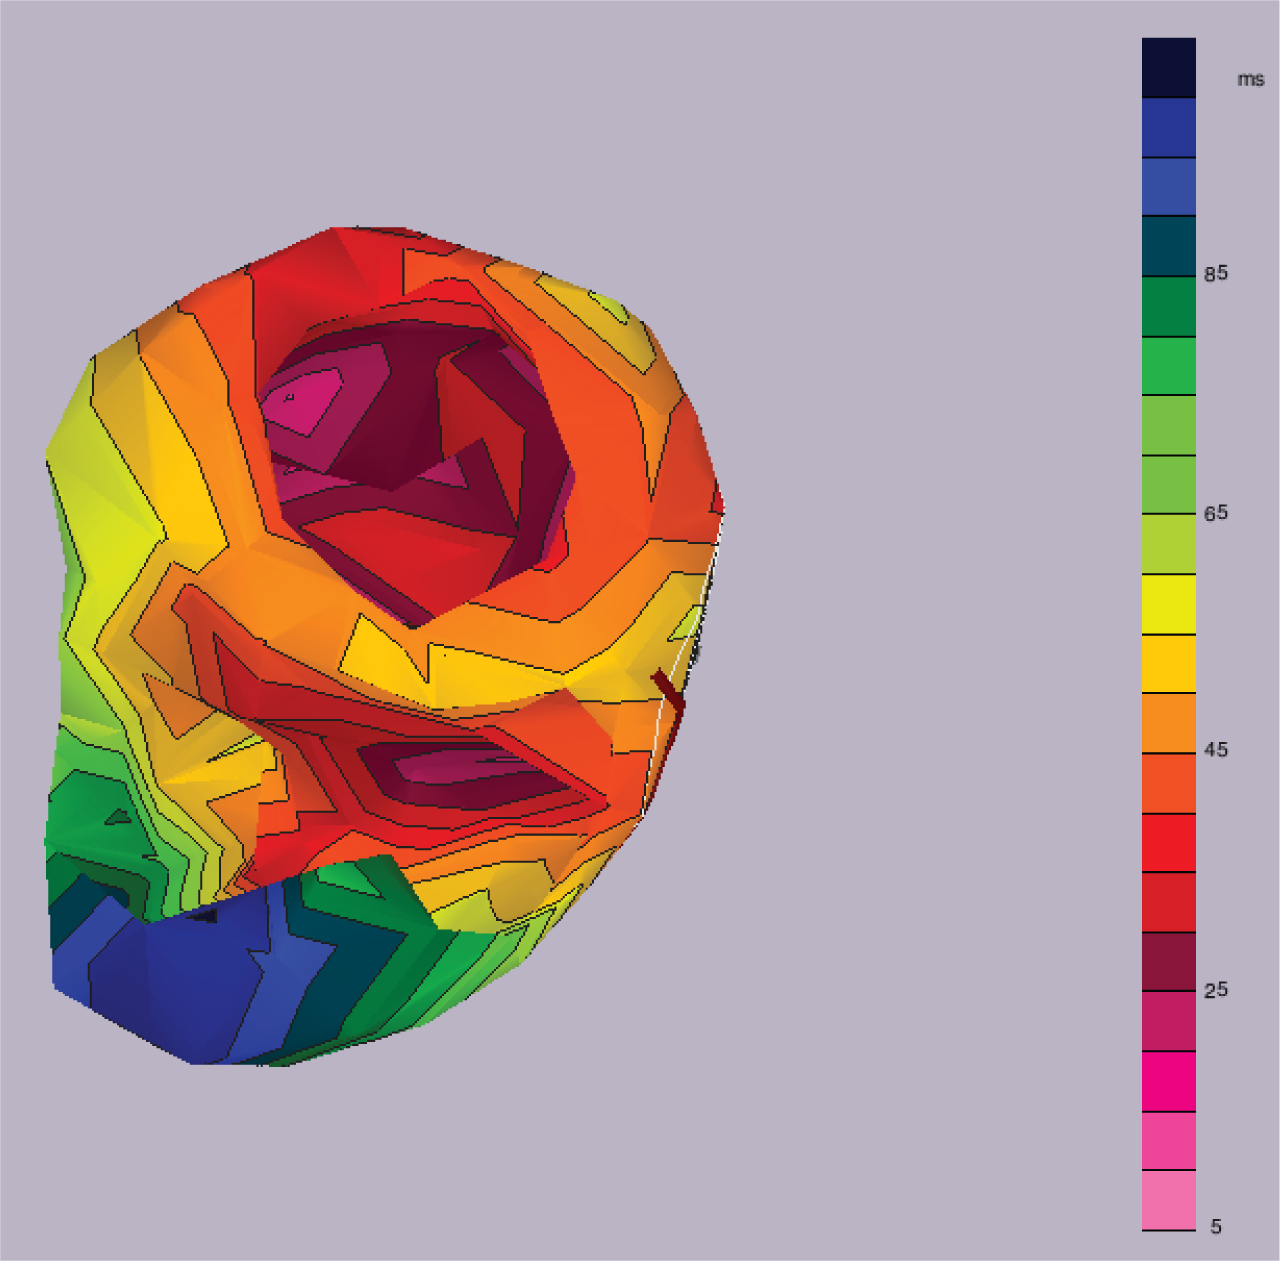
\includegraphics[width=.95\linewidth]{Figures/1_1_actTimes_1.png}
		\caption{}
		
	\end{subfigure}%
	\begin{subfigure}{.5\textwidth}
		\centering
		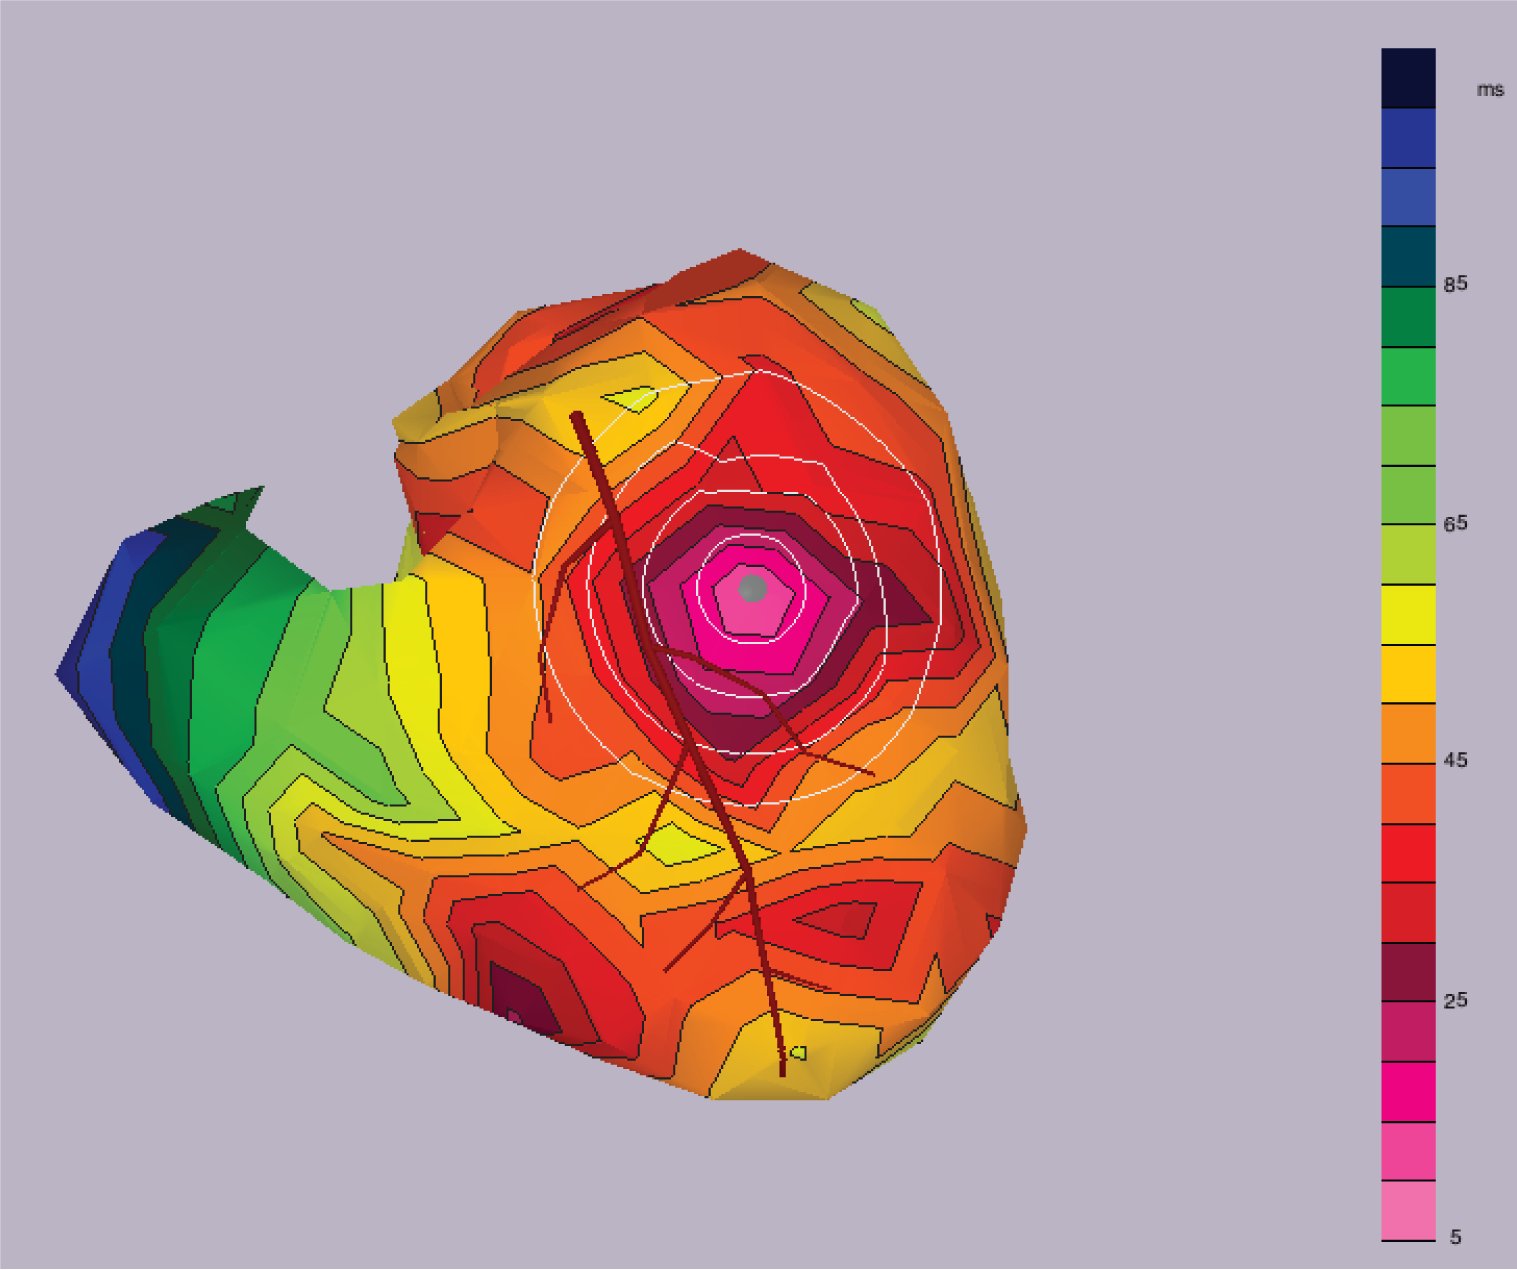
\includegraphics[width=.95\linewidth]{Figures/1_1_actTimes_2.png}
		\caption{}
		
	\end{subfigure}
	\caption{Activation times mapped onto the endocardium and epicardium. The color bar shows the spread of activation times. The heart is viewed from the atrial ventricular plane looking into the ventricles (a), and on the anterior surface (b).}
	\label{1_1_actTimes}
\end{figure}

\begin{figure}[H]
	\centering
	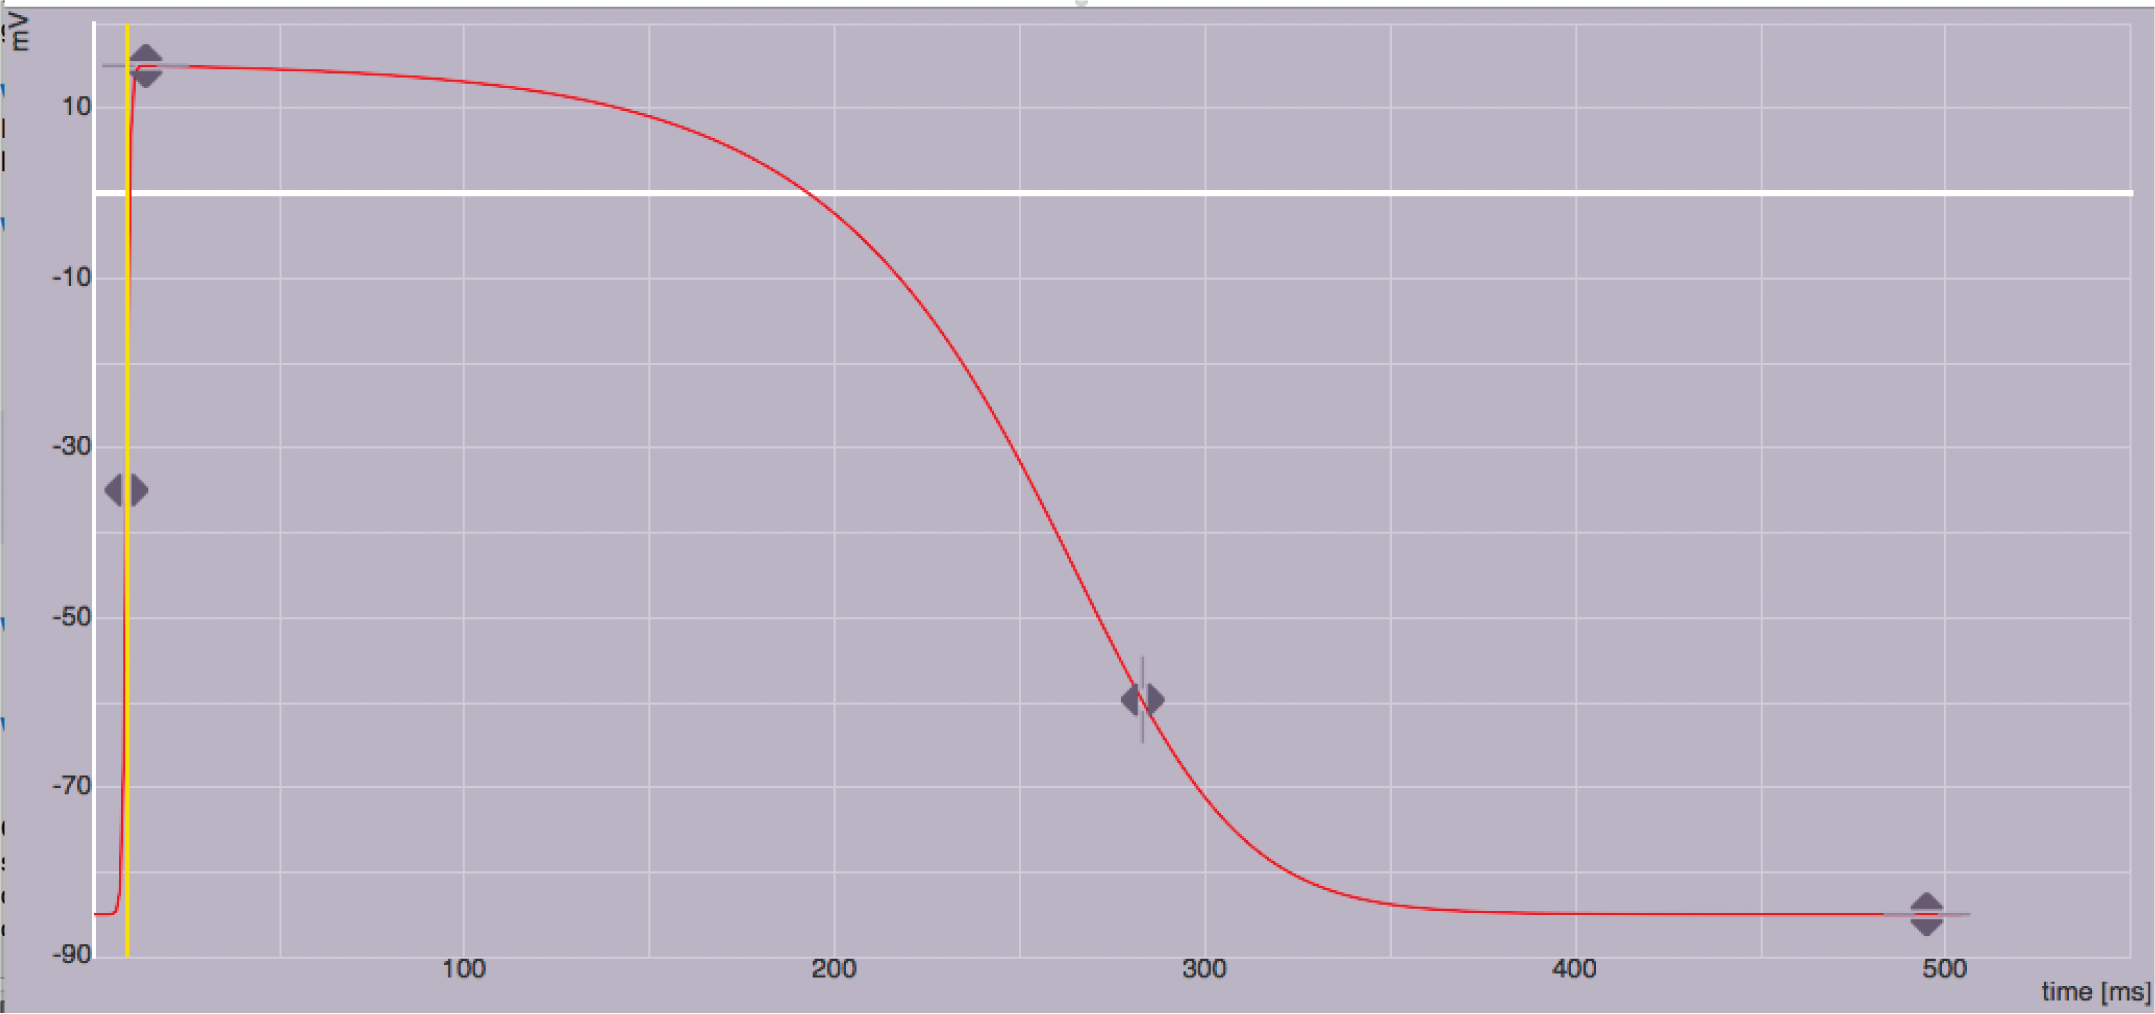
\includegraphics[width=.95\linewidth]{Figures/1_1_actpotential.png}

	\caption{Membrane potential of the node highlighted in Figure~\ref{1_1_actTimes}.b}
	\label{1_1_vm}
\end{figure}

\subsection{1.2: }


\begin{figure}[H]
	\begin{subfigure}{.5\textwidth}
		\centering
		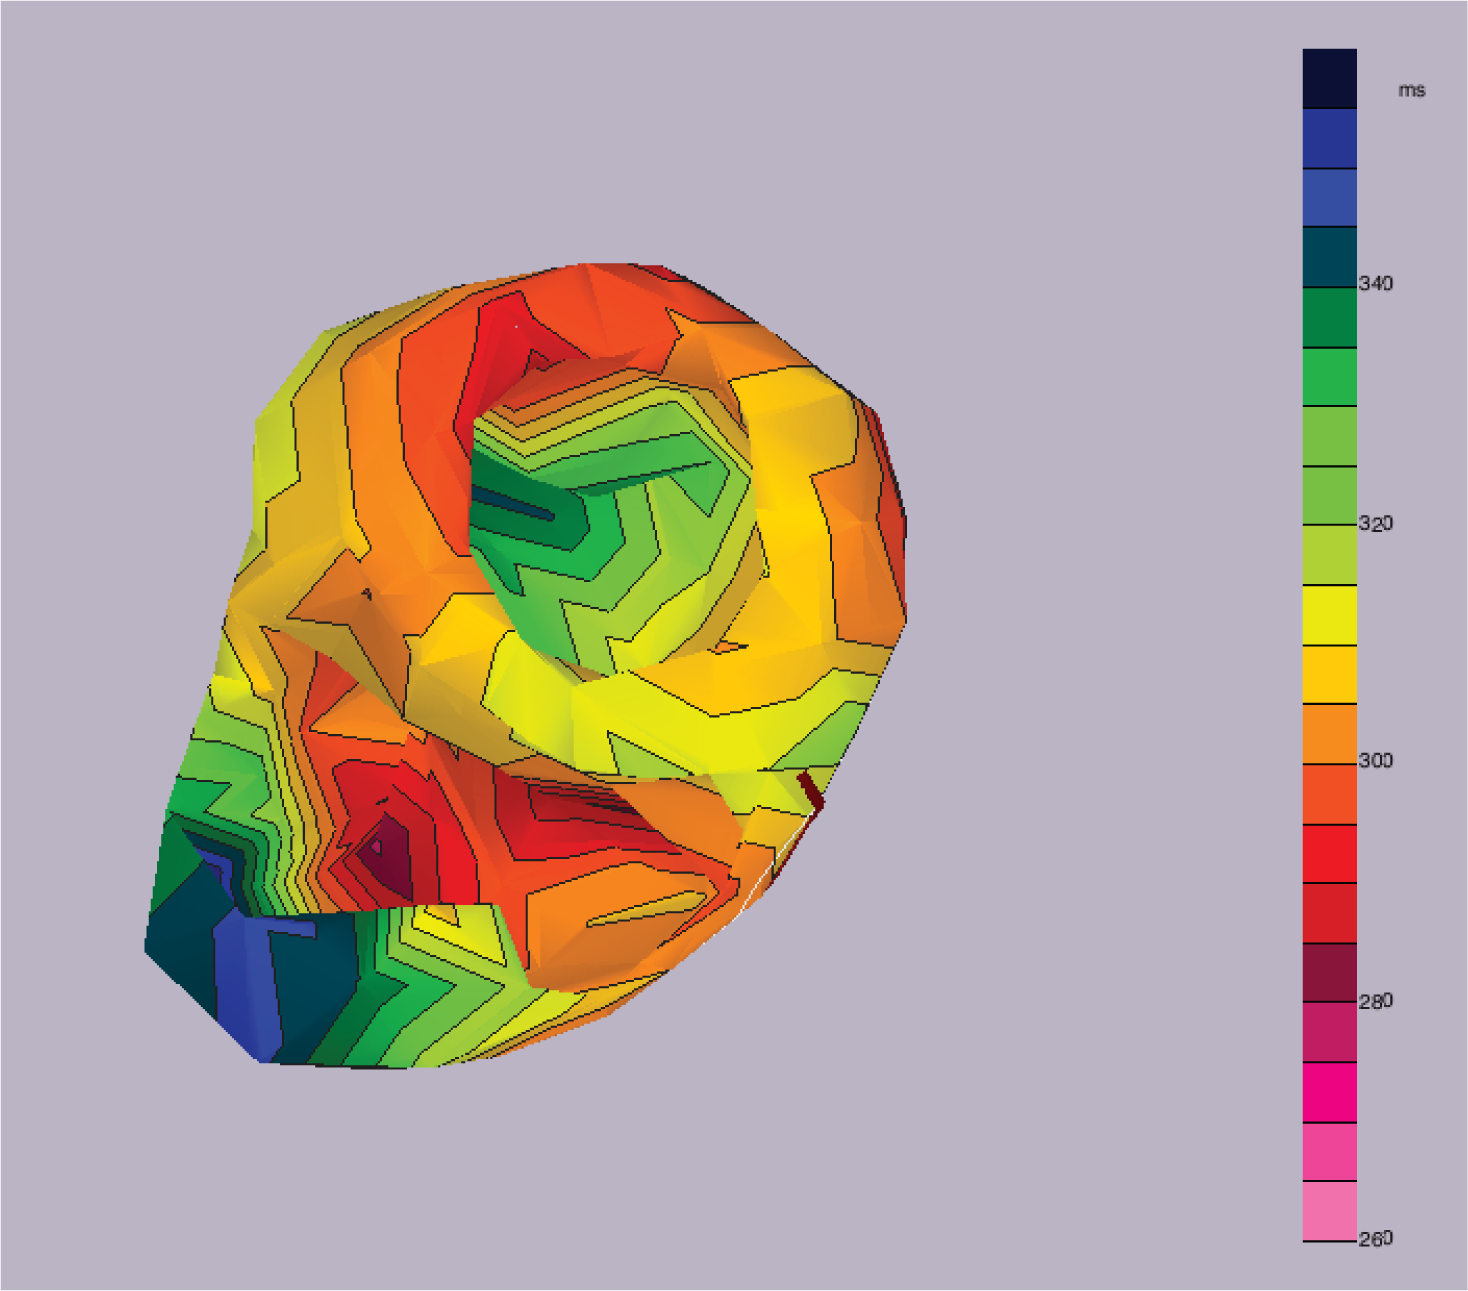
\includegraphics[width=.95\linewidth]{Figures/1_2_recTimes_1.png}
		\caption{}
		
	\end{subfigure}%
	\begin{subfigure}{.5\textwidth}
		\centering
		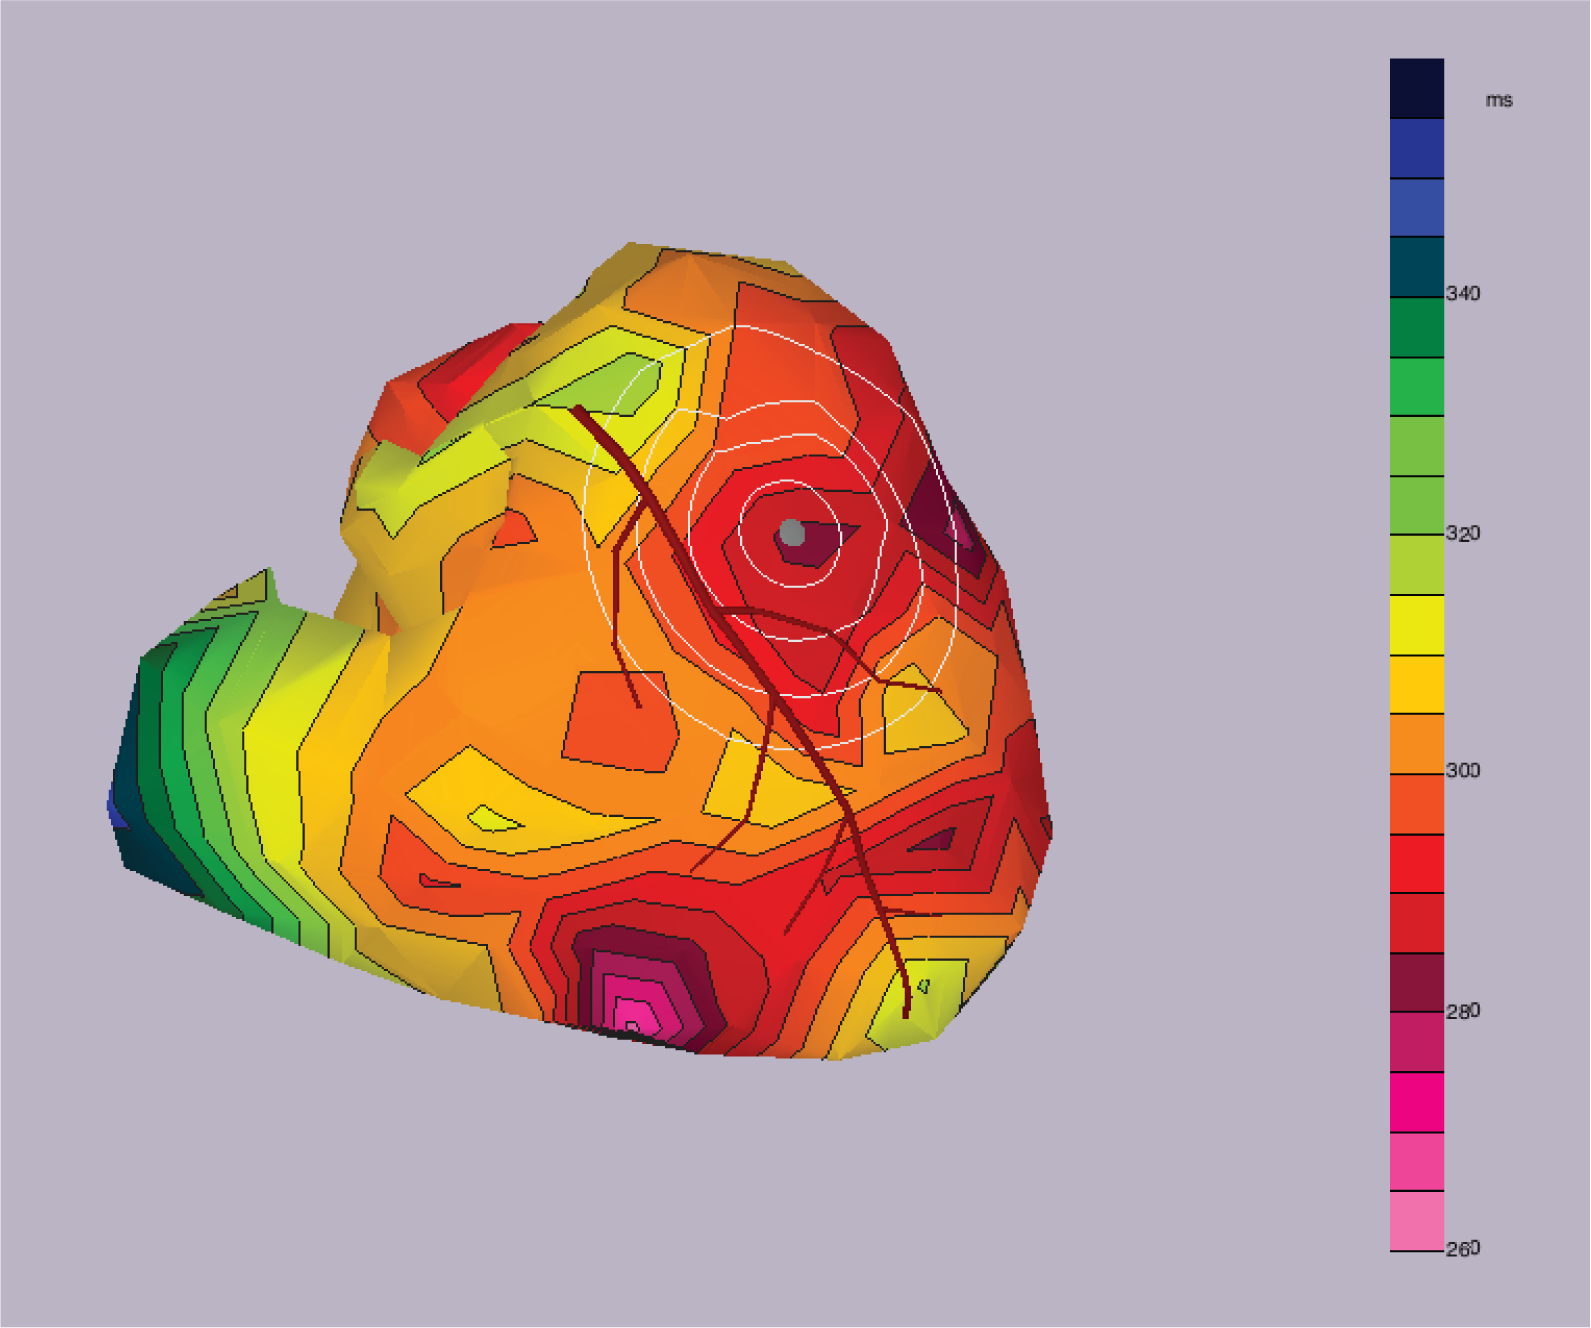
\includegraphics[width=.95\linewidth]{Figures/1_2_recTimes_2.png}
		\caption{}
		
	\end{subfigure}
	\caption{Activation times mapped onto the endocardium and epicardium. The color bar shows the spread of activation times. The heart is viewed from the atrial ventricular plane looking into the ventricles (a), and on the anterior surface (b).}
	\label{1_2_recTimes}
\end{figure}

\begin{figure}[H]
	\centering
	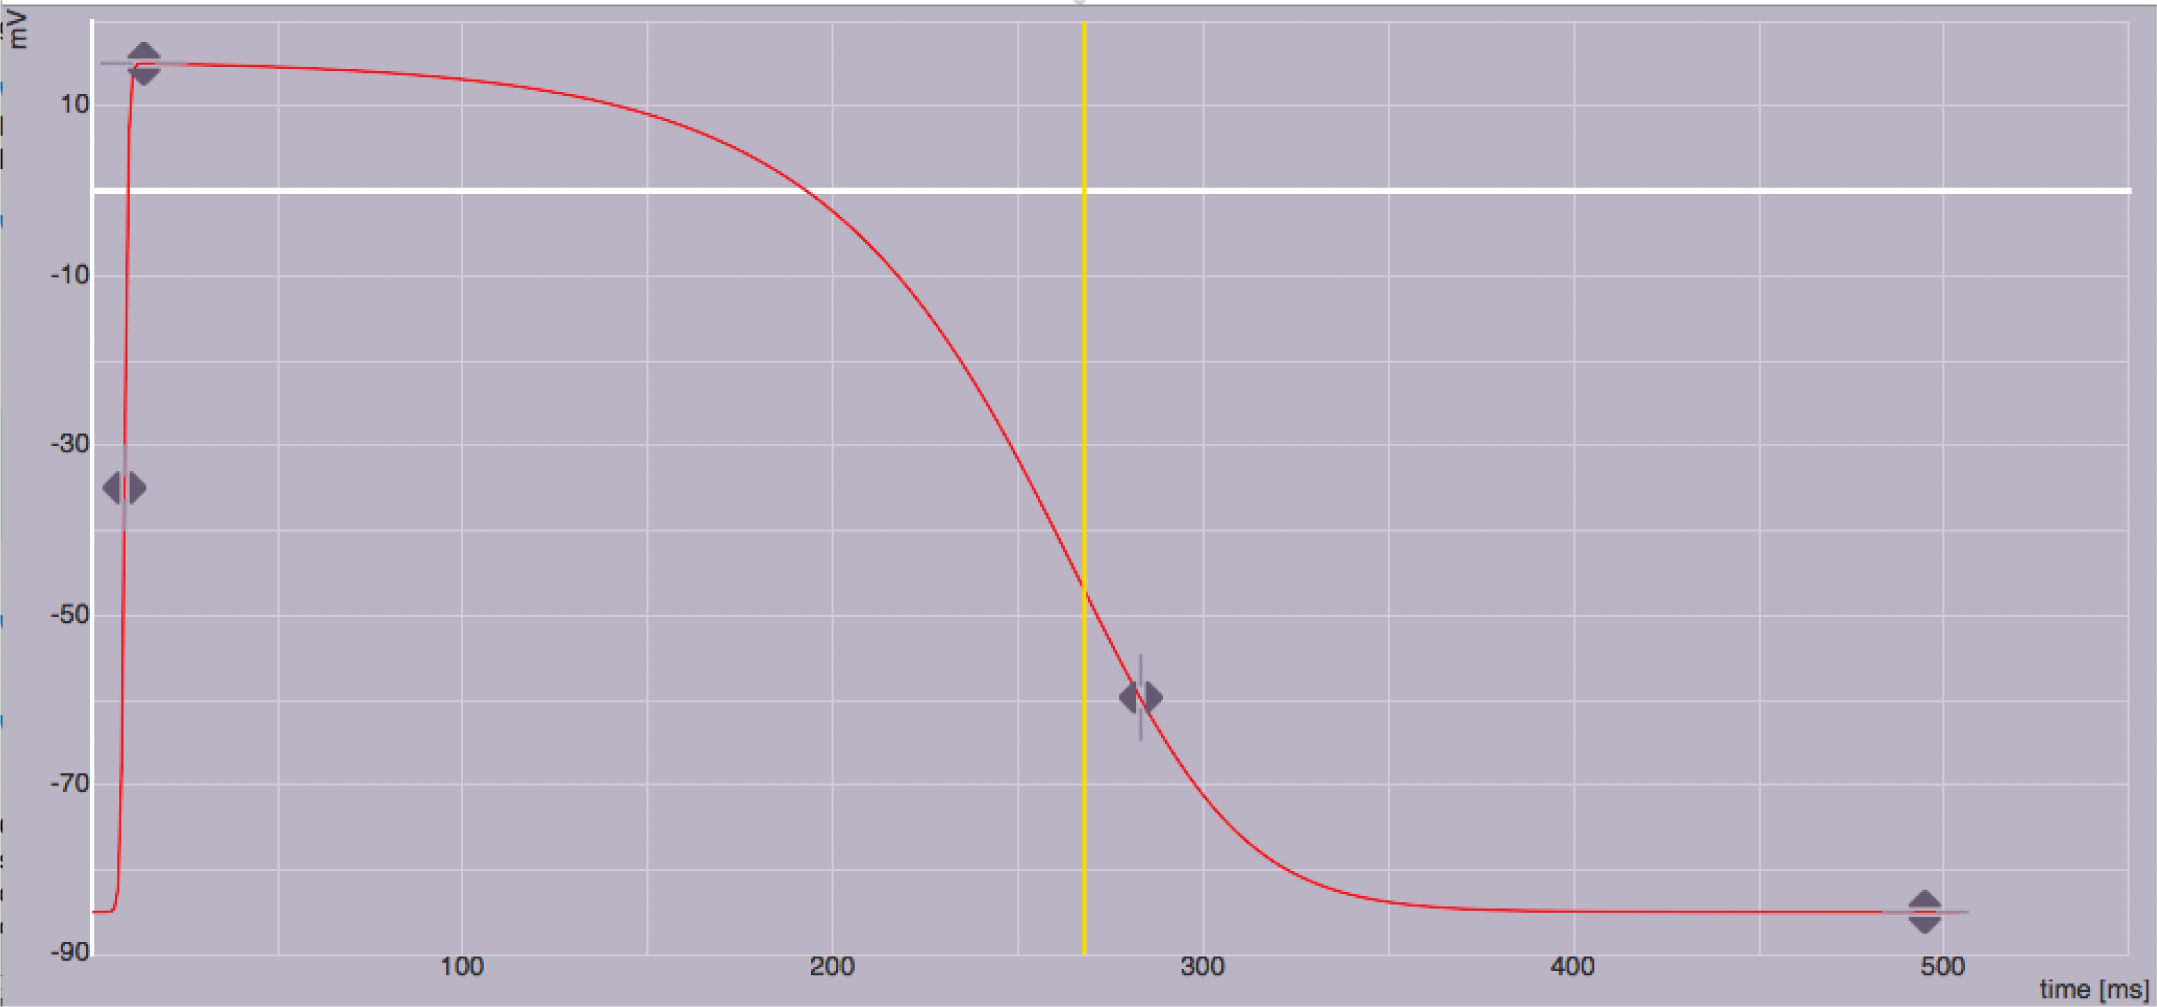
\includegraphics[width=.95\linewidth]{Figures/1_2_actpotential.png}
	
	\caption{Membrane potential of the node highlighted in Figure~\ref{1_1_actTimes}.b}
	\label{1_2_vm}
\end{figure}


\subsection{1.3: }
\begin{figure}[H]
	\begin{subfigure}{.75\textwidth}
		\centering
		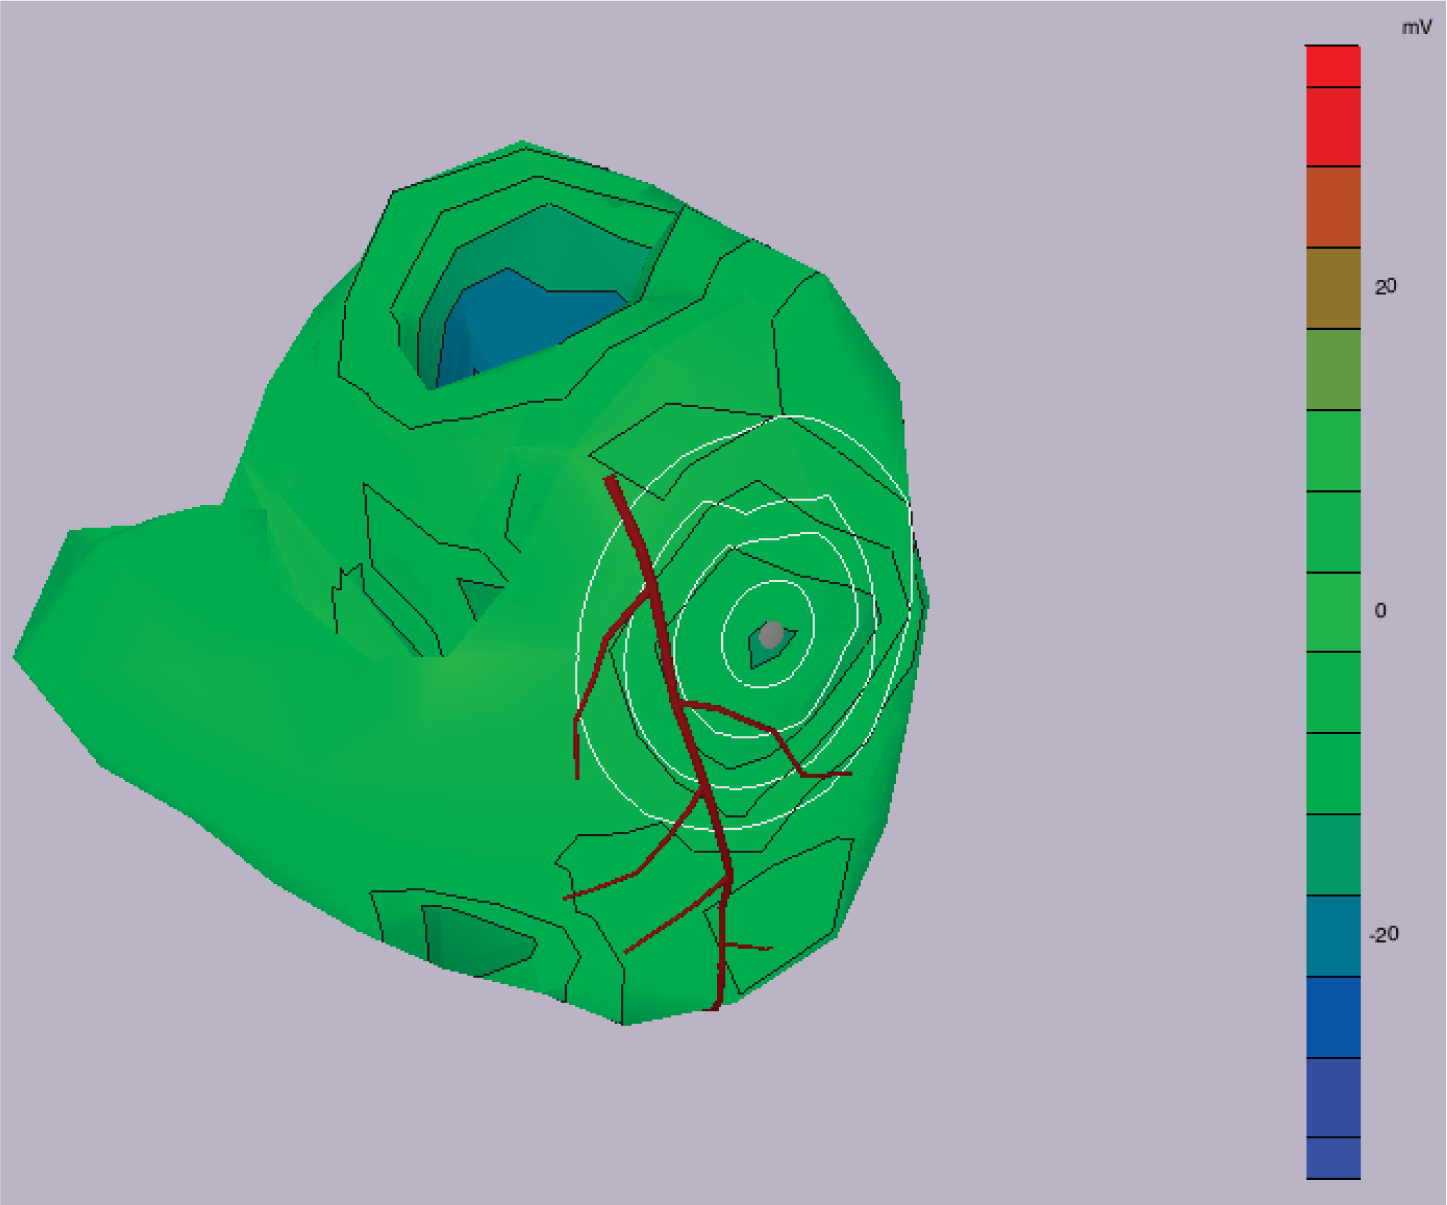
\includegraphics[width=.95\linewidth]{Figures/1_3_pot_1.png}
		\caption{}
		
	\end{subfigure}%
\\
	\begin{subfigure}{.95\textwidth}
		\centering
		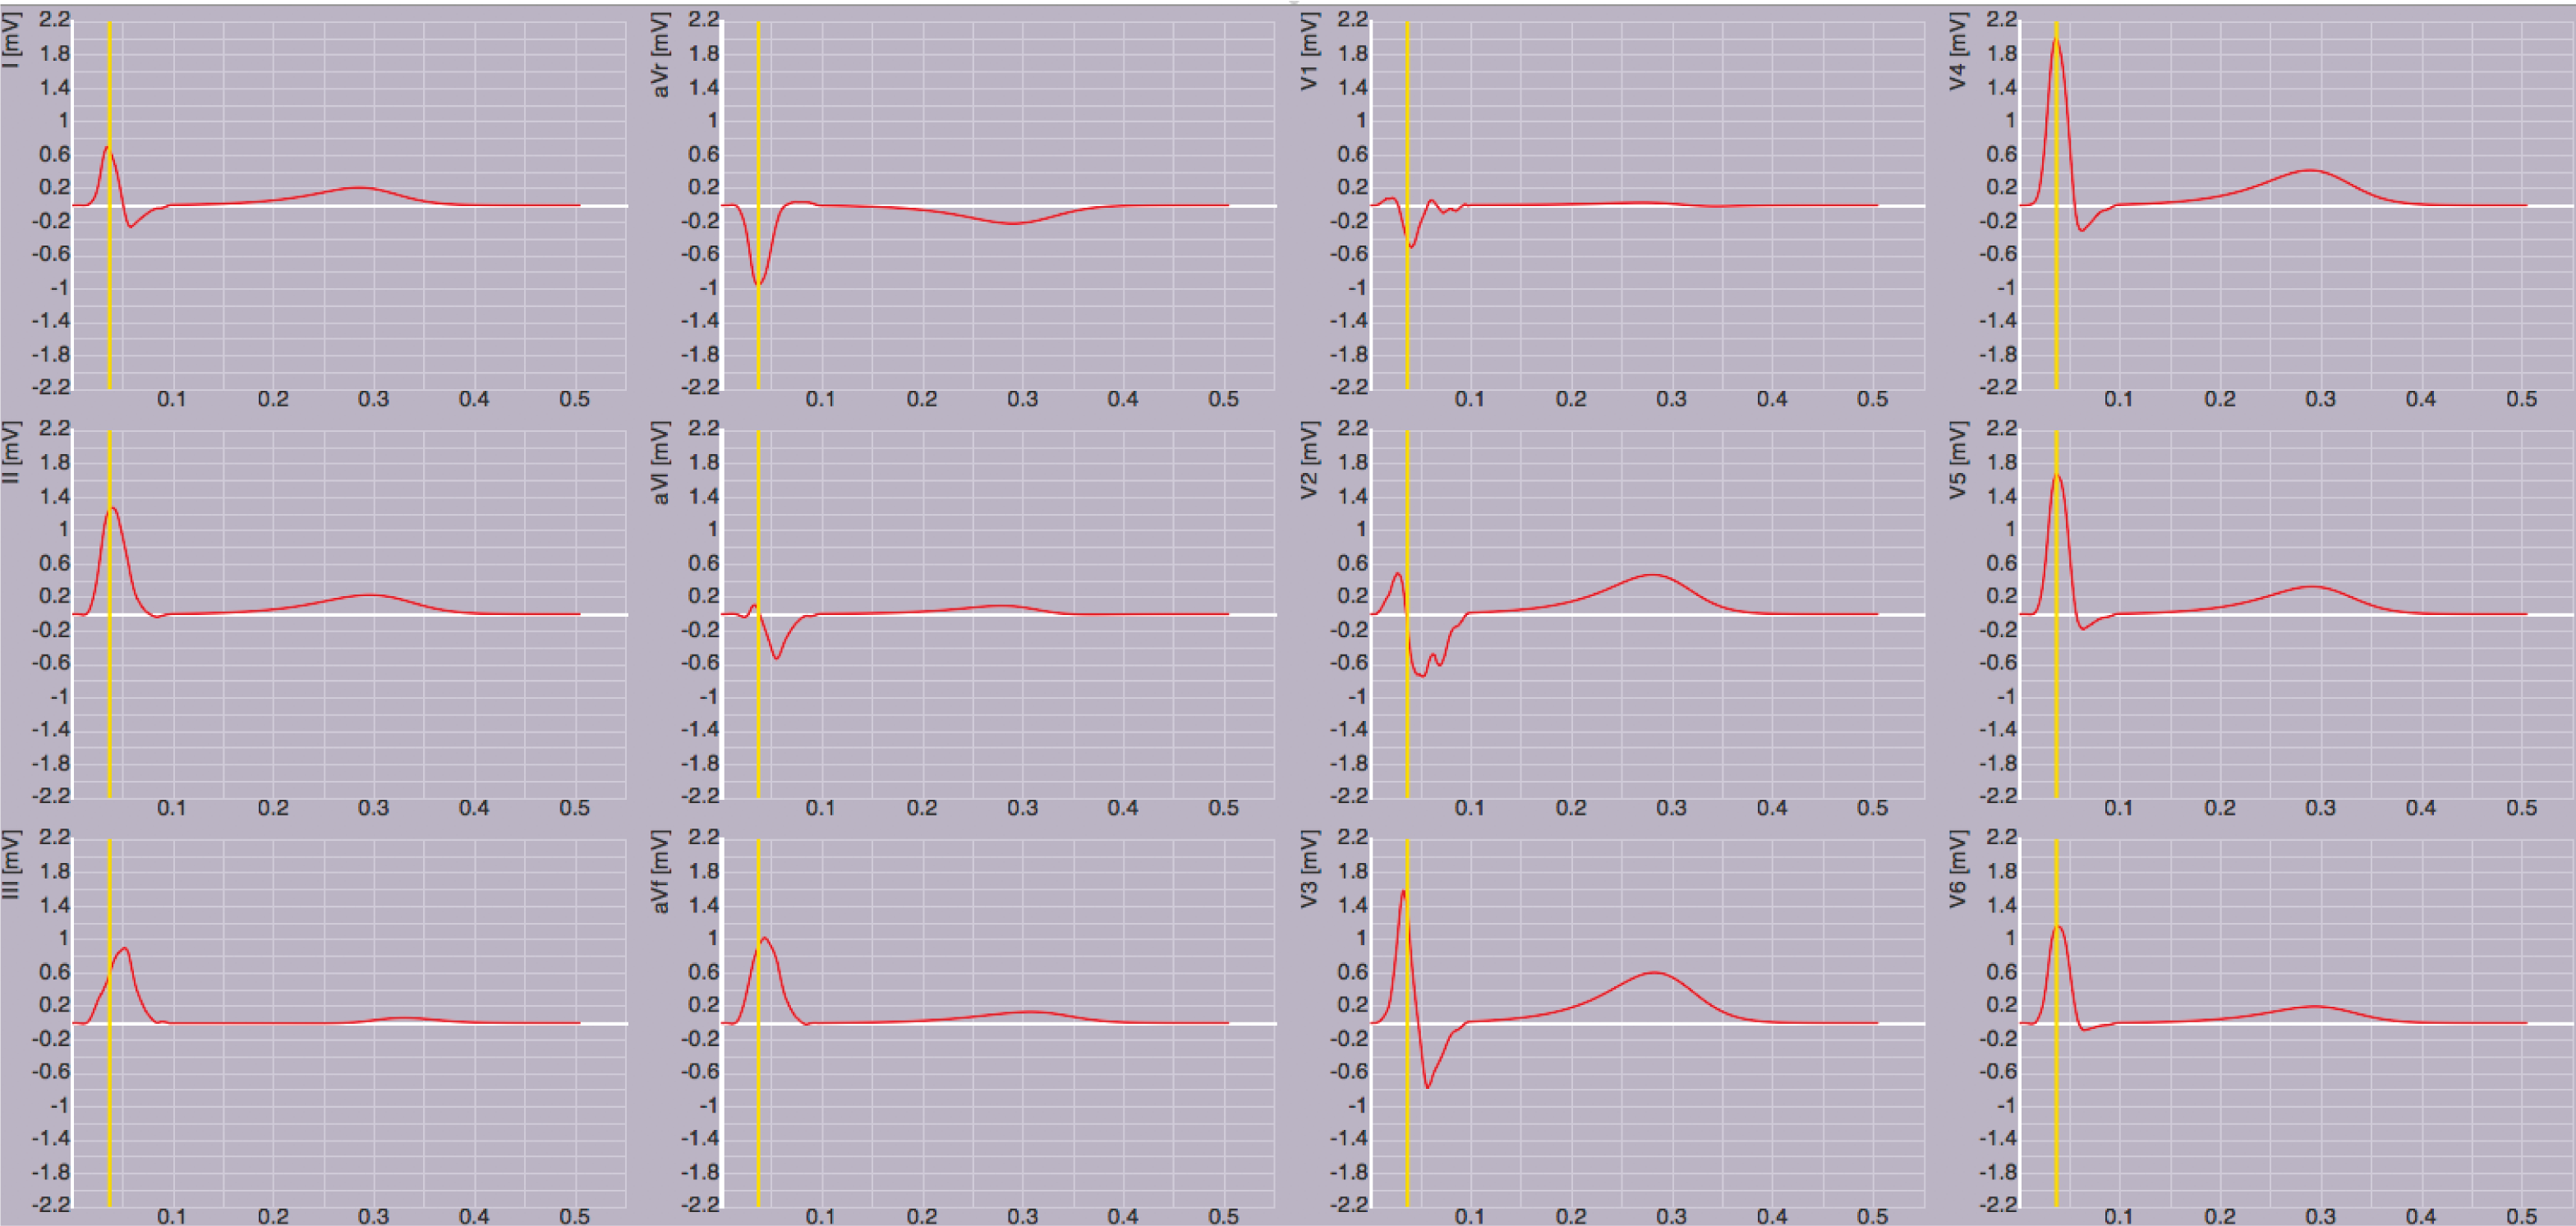
\includegraphics[width=.95\linewidth]{Figures/1_3_ecg_1.png}
		\caption{}
		
	\end{subfigure}
	\caption{Activation times mapped onto the endocardium and epicardium. The color bar shows the spread of activation times. The heart is viewed from the atrial ventricular plane looking into the ventricles (a), and on the anterior surface (b).}
	\label{1_3_1}
\end{figure}
\begin{figure}[H]
	\begin{subfigure}{.75\textwidth}
		\centering
		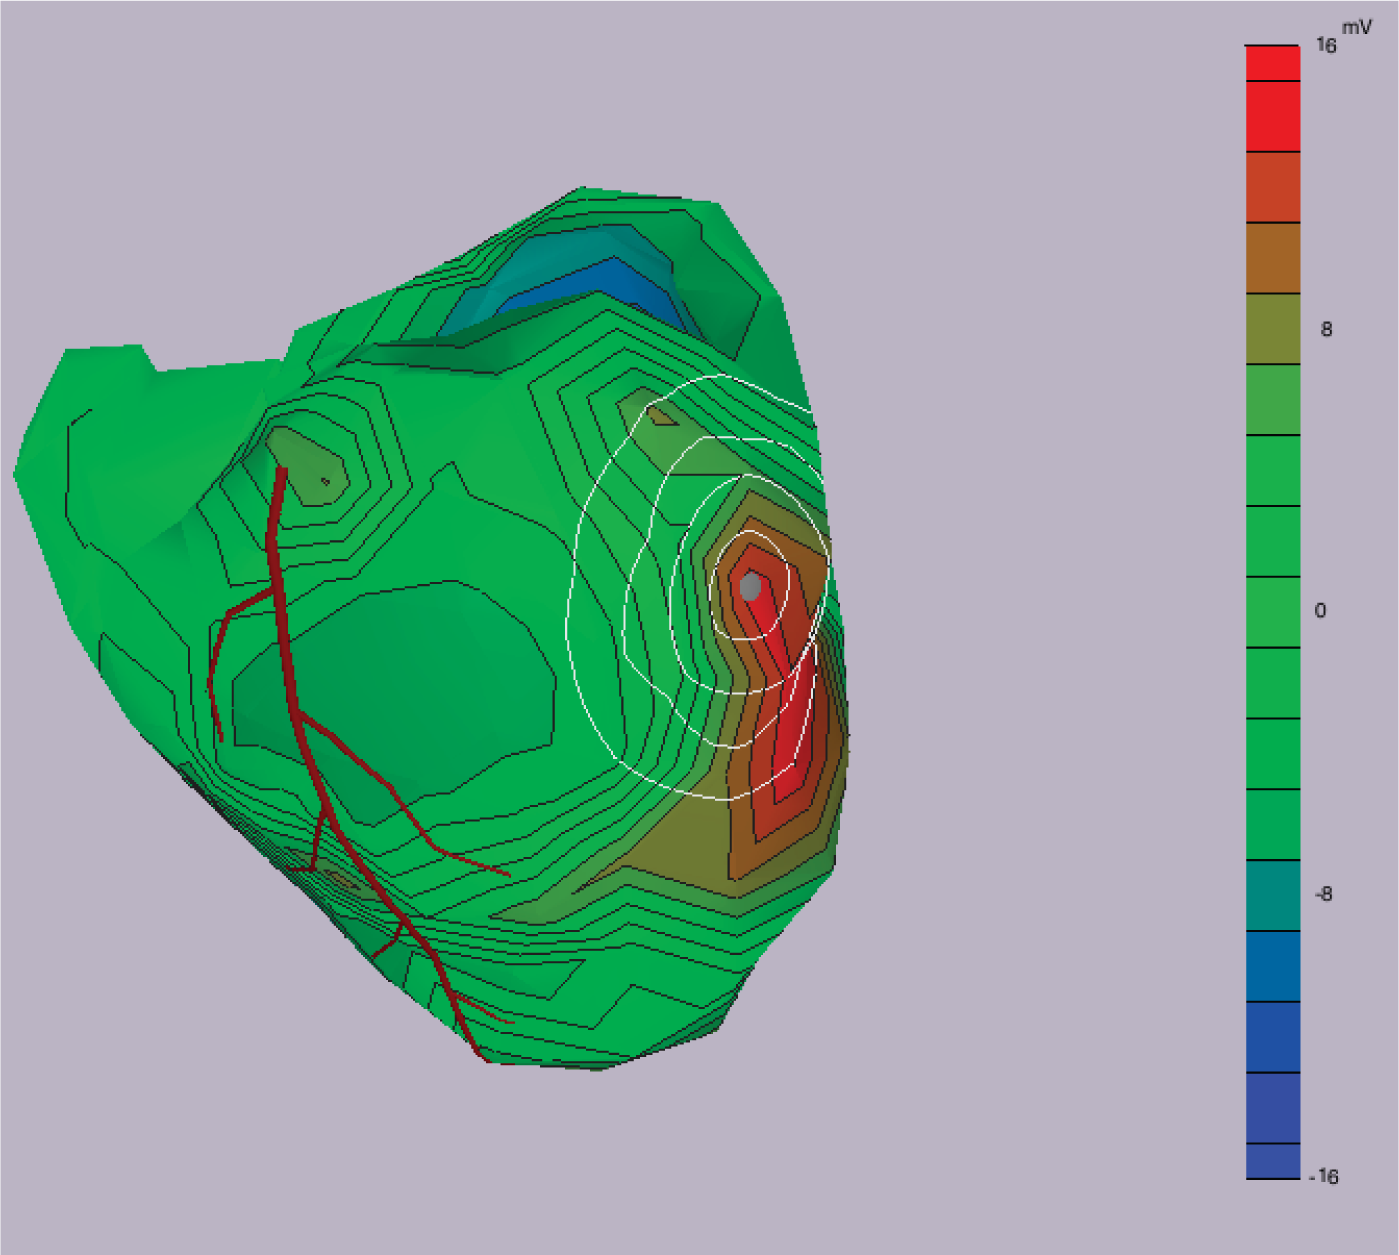
\includegraphics[width=.95\linewidth]{Figures/1_3_pot_2.png}
		\caption{}
		
	\end{subfigure}%
\\
	\begin{subfigure}{.95\textwidth}
		\centering
		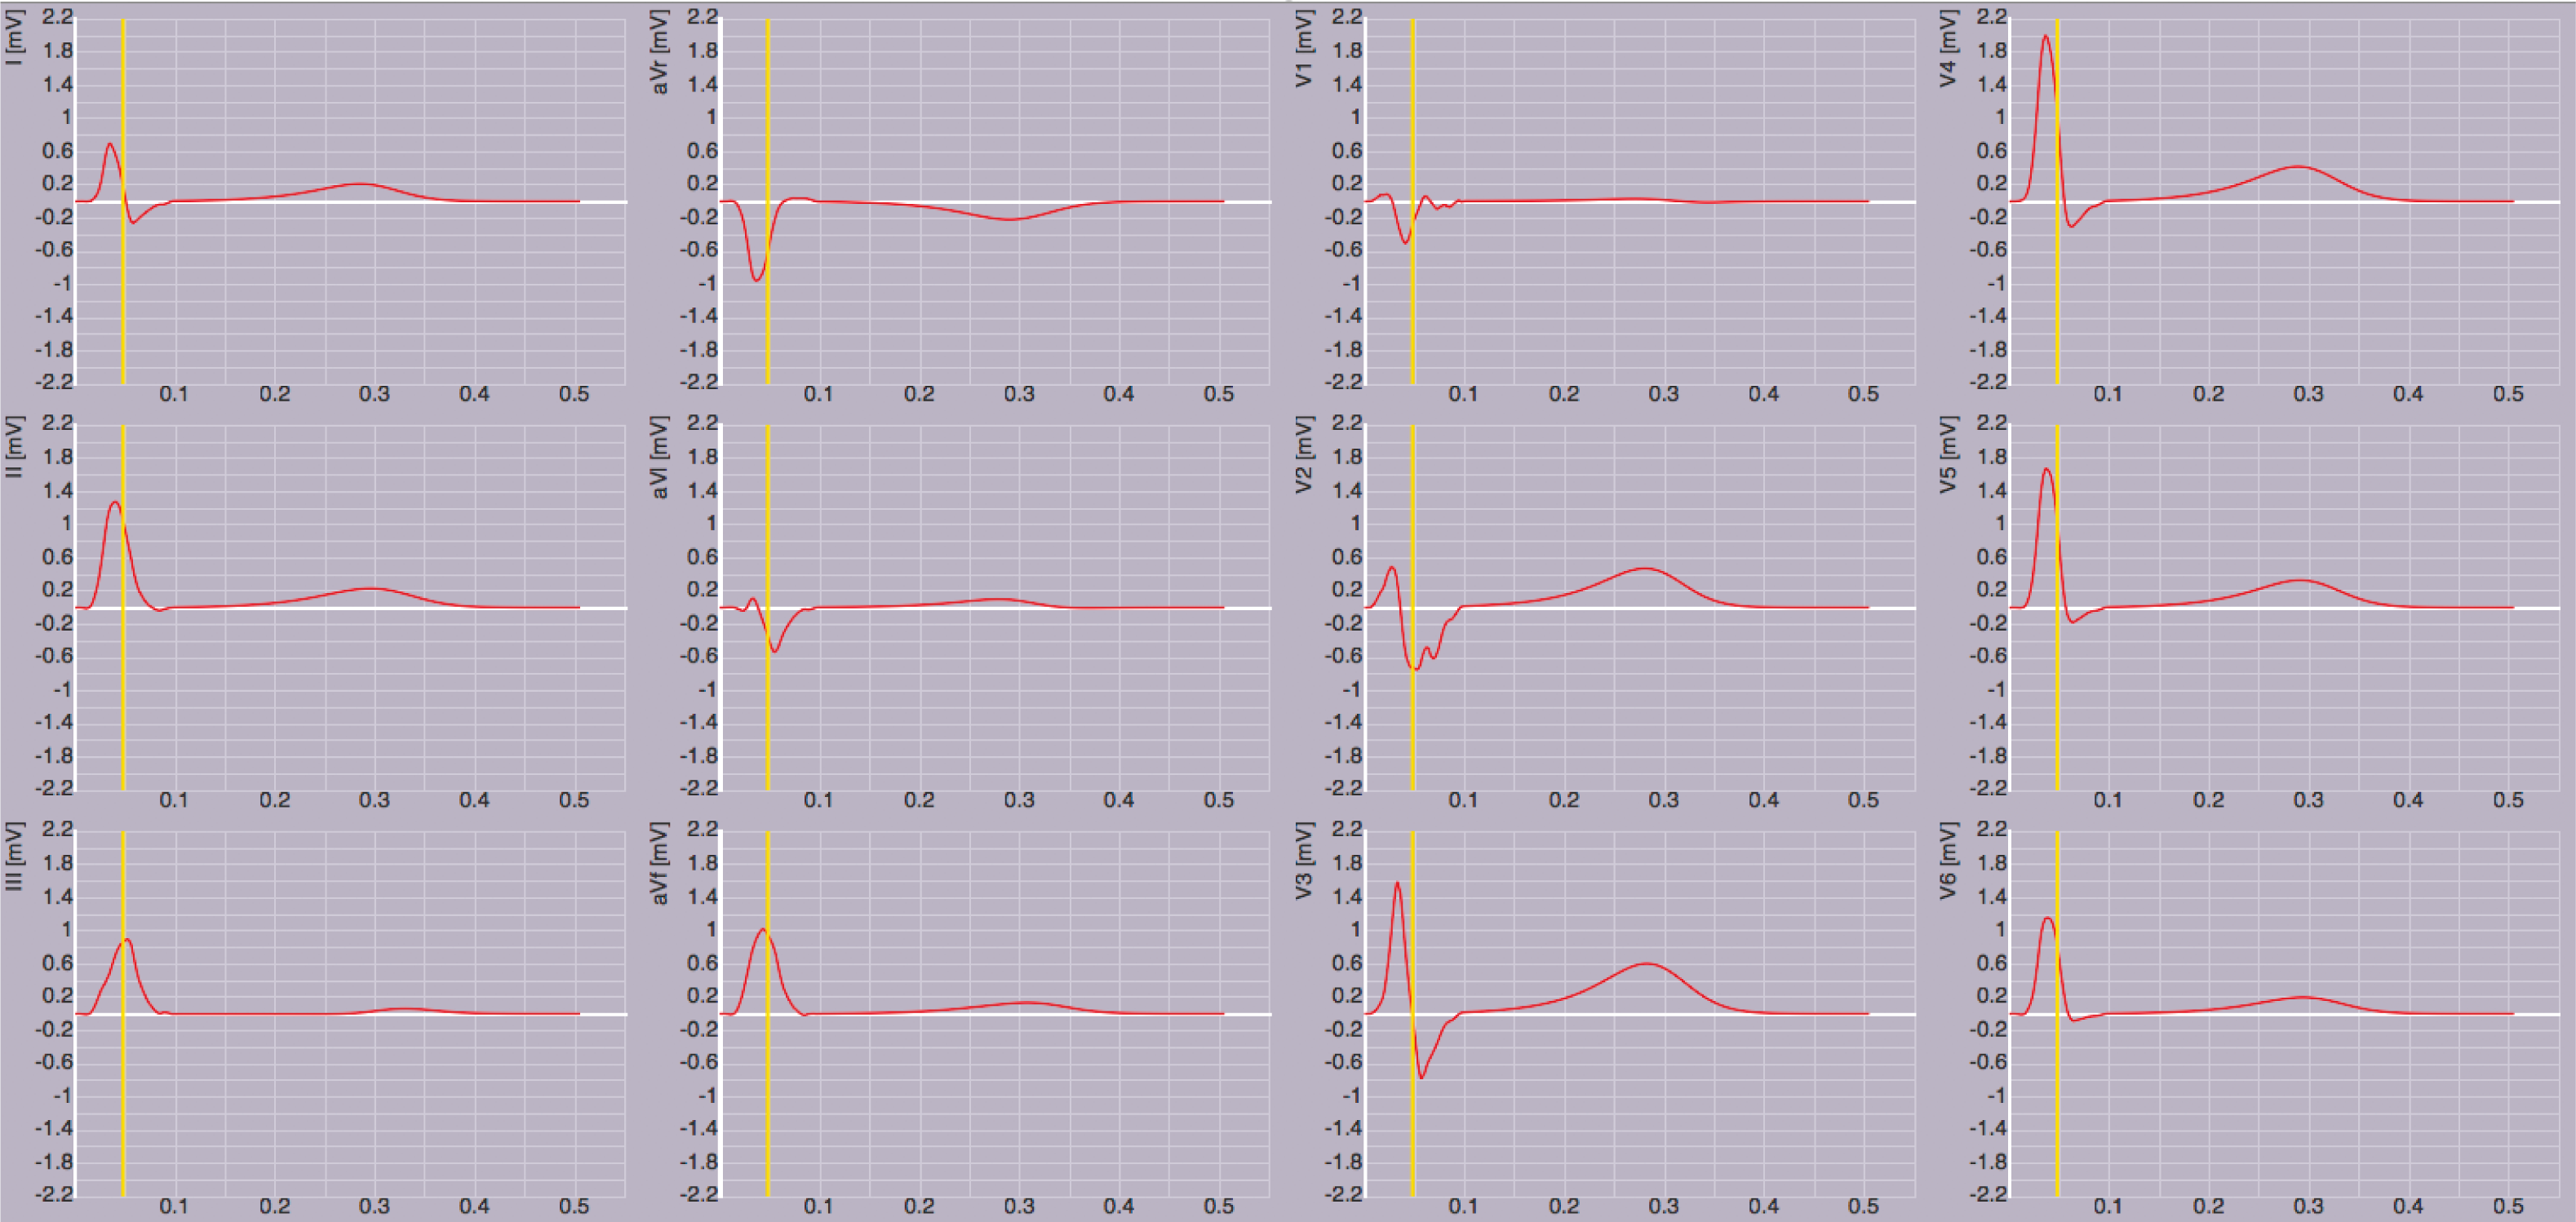
\includegraphics[width=.95\linewidth]{Figures/1_3_ecg_2.png}
		\caption{}
		
	\end{subfigure}
	\caption{Activation times mapped onto the endocardium and epicardium. The color bar shows the spread of activation times. The heart is viewed from the atrial ventricular plane looking into the ventricles (a), and on the anterior surface (b).}
	\label{1_3_2}
\end{figure}


\subsection{2.1: }
\begin{figure}[H]
	\begin{subfigure}{.95\textwidth}
		\centering
		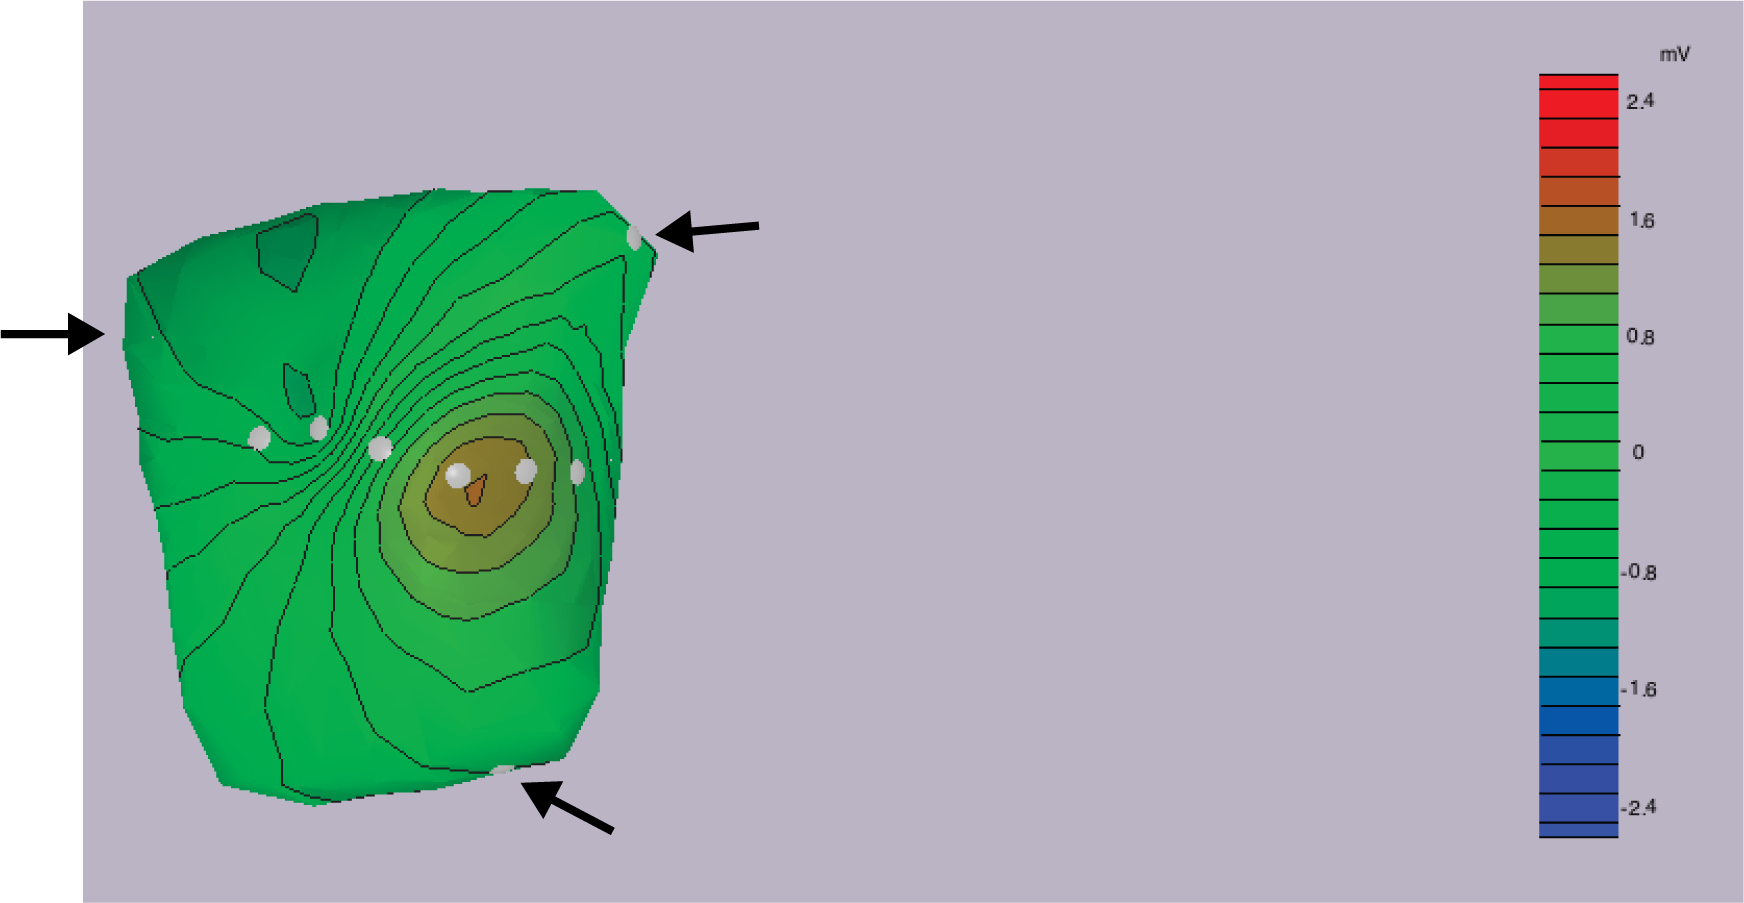
\includegraphics[width=.95\linewidth]{Figures/2_1_bsp.png}
		\caption{}
		
	\end{subfigure}%
	\\
	\begin{subfigure}{.95\textwidth}
		\centering
		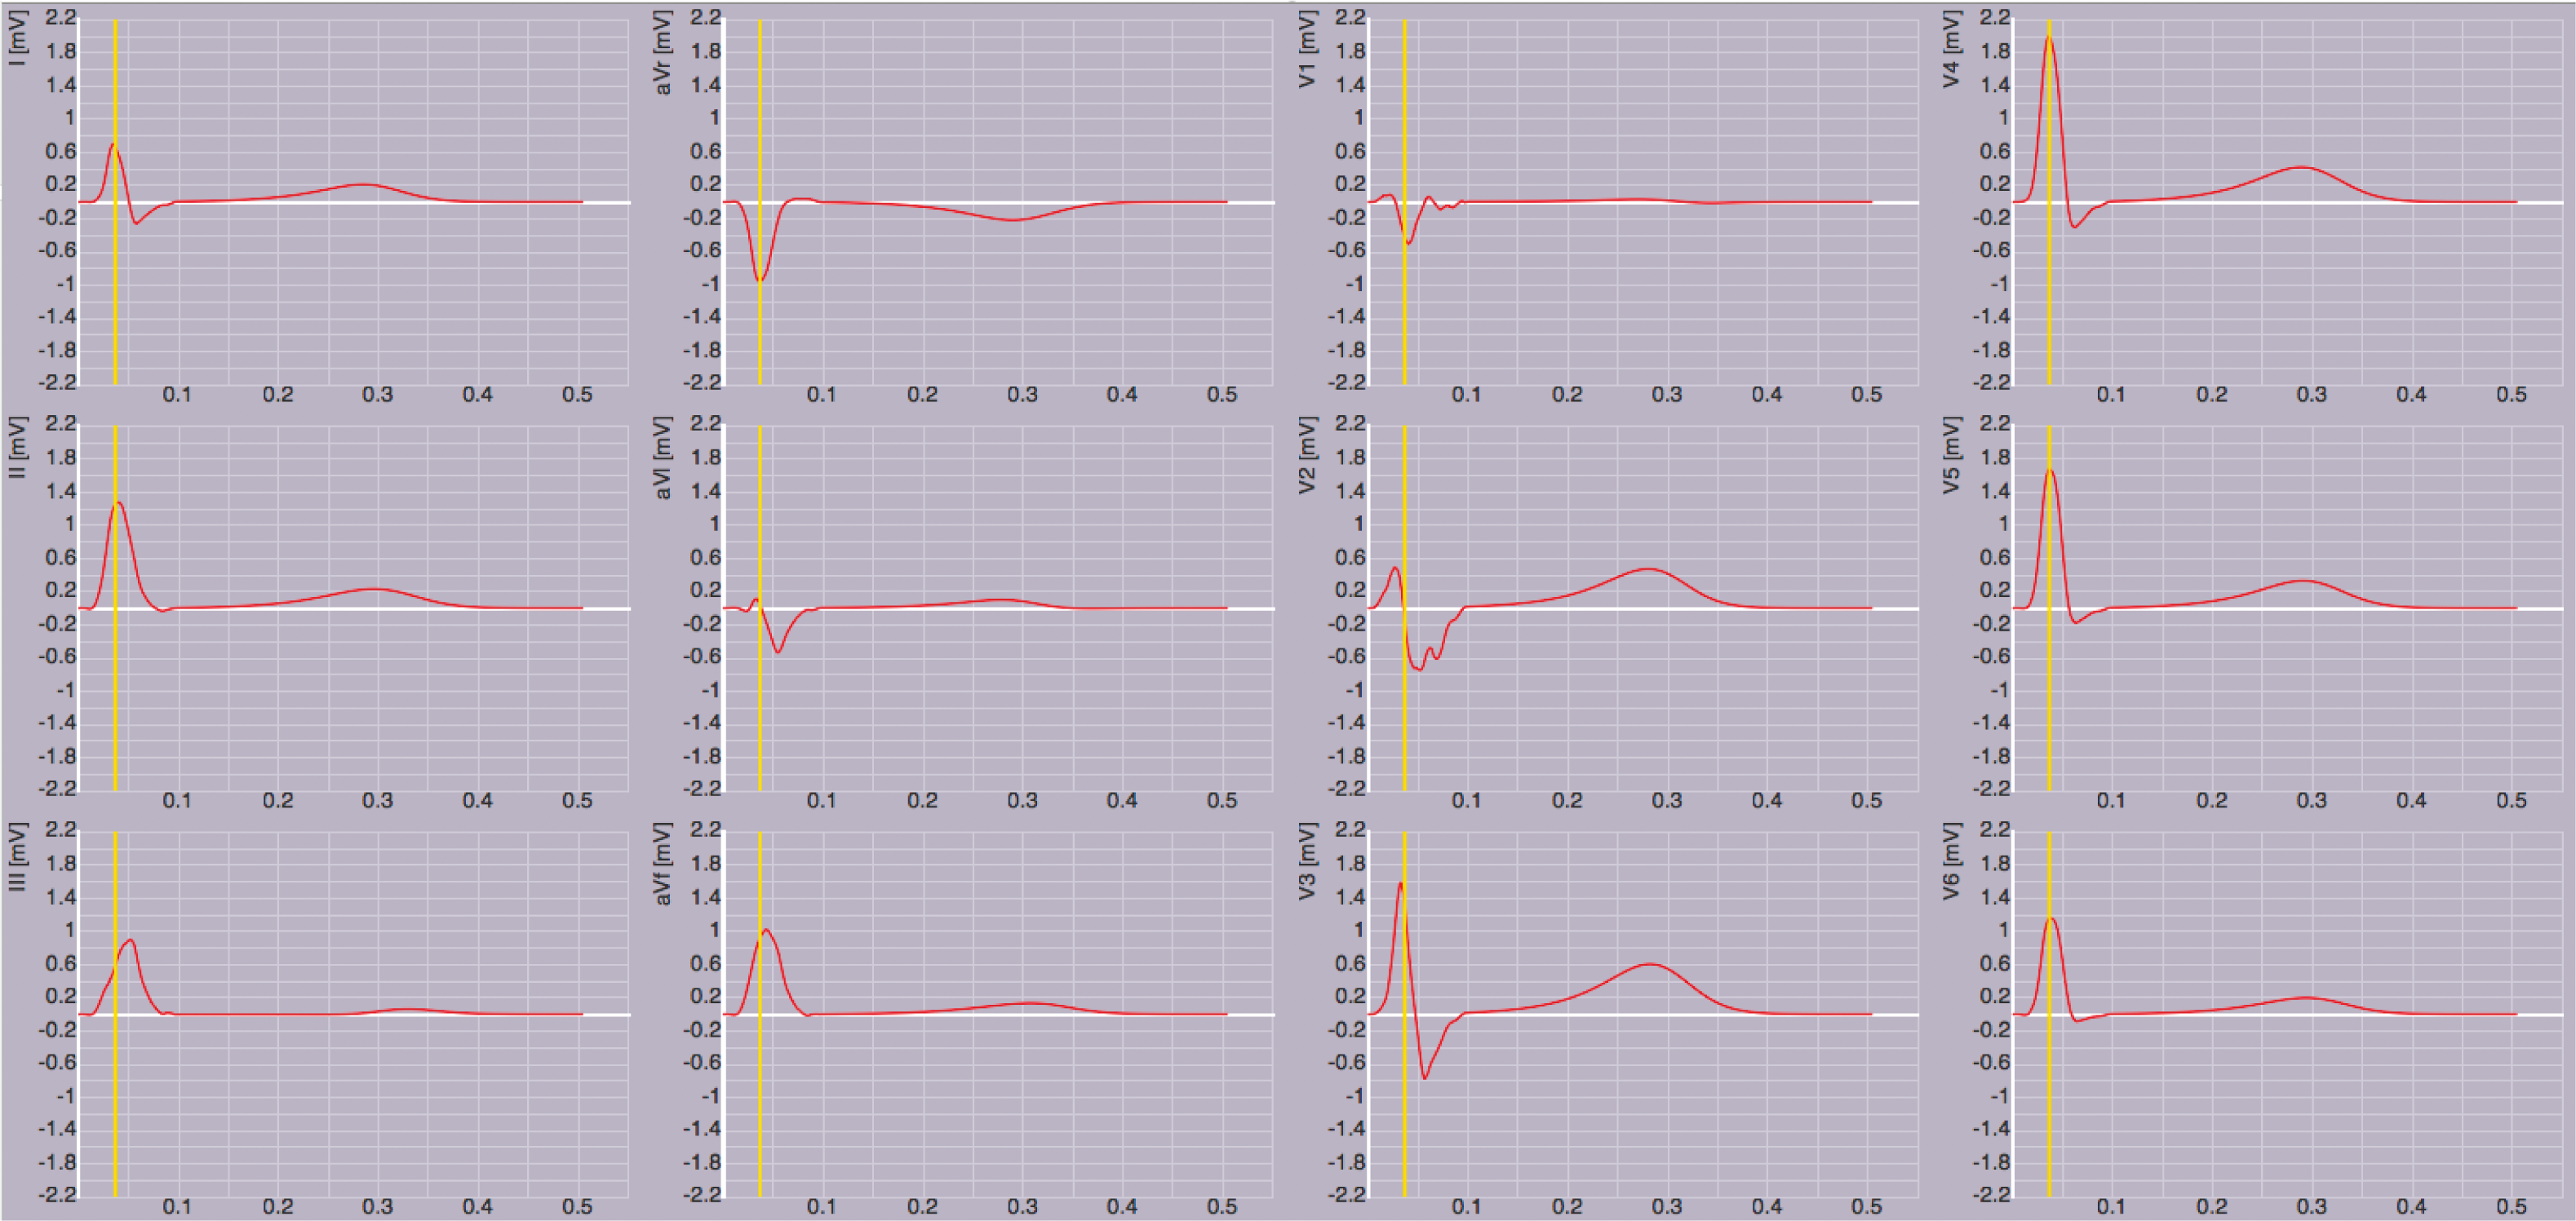
\includegraphics[width=.95\linewidth]{Figures/2_1_ecg.png}
		\caption{}
		
	\end{subfigure}
	\caption{Activation times mapped onto the endocardium and epicardium. The color bar shows the spread of activation times. The heart is viewed from the atrial ventricular plane looking into the ventricles (a), and on the anterior surface (b).}
	\label{2_1}
\end{figure}


\subsection{2.2: }


\subsection{2.3: }


\section{Discussion and Conclusions}


Clearly the ECGSim tool deonstrates the practicality and flexibility of a simulation tool for the investigation of the effects of different cardiac source behaviors and conditions ont he resulting body surface ECGs. This simulation environment has the advantage of being free, quick, and flexible. Using this tool researchers can vary several parameters that are impractcal or impossible to access during even a large anmial or cell culture experimental preparation, such as directly modifying the actionpotentials of cardiac tissue. This unparalelled level of control allows for very specific and detailed analysis to be performed on a scale that is otherwise impossible. However, simulations do have downsides. One obvious shortfall of ECGSim is the lack of atria in the propagation model. Without these the ECG lack the caracteristic P wave, and physiological conditions having to do with atrial activity, and ventricular atrial interplay cannot be assessed.  Additionally all models make simplifying assumptions in order to make them computationally feasible. This however limits their translatability to real physiology as the the model does not fully represent physiological function. For example the ECGSim geometries do not allow for changes at a cellular scale nor do they model propagation. These limitations prevent analysis of changes to parameters in these areas, and thus limit the scope of the simulation's use. 

%%%%%%%%%%%%%%%%%% Correct Bibliography Style

%\bibliography{/Users/jbergquist/Documents/BibTex/Library}
%\bibliographystyle{ieeetr}


\end{document}








